\documentclass[tikz]{standalone}
\usepackage{pgfplots}
\pgfplotsset{compat=1.15}
\usepackage{mathrsfs}
\usetikzlibrary{arrows,calc}
\usepackage{tkz-euclide}

\pagestyle{empty}

\definecolor{AngleClr}{rgb}{0,0.39215686274509803,0}
\definecolor{ShapeClr}{rgb}{0.6,0.2,0}

\begin{document}

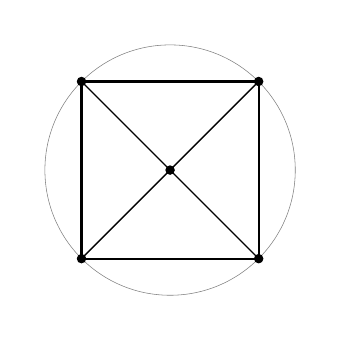
\begin{tikzpicture}[scale=.75]
\tkzSetUpLine[line width=1pt,color=black]
\tkzSetUpPoint[fill=black]

\tkzDefPoints{0/0/A,0/3/B,3/3/C,3/0/D}

\tkzDefMidPoint(A,B) \tkzGetPoint{M1}
\tkzDefMidPoint(C,D) \tkzGetPoint{M2}
\tkzDefMidPoint(B,C) \tkzGetPoint{M3}
\tkzDefMidPoint(D,A) \tkzGetPoint{M4}

% \tkzFillPolygon[fill=white](P1,P2,P3,P4,P5,P6,P7,P8)

% Step 2
\tkzDrawSegments[line width=0.5pt,color=black](A,C B,D)

% Step 3
\tkzInterLL(A,C)(B,D) \tkzGetPoint{O}
\tkzDrawCircle(O,A)

\begin{scope}[opacity=0.0]
\tkzDrawSegments[line width=0.5pt,color=black,dashed,dash pattern=on 1pt off 1.75pt,add=0.3 and 0.3](M1,M2 M3,M4)
\end{scope}

\tkzDrawPolygon[color=black,line width=0.8pt](A,B,C,D)
\tkzDrawPoints[size=3](A,B,C,D,O)


\end{tikzpicture}

\end{document}
